


% TODO replace \delta with \partial derp MAYBE




% Compiling

%     You need to include your .tex source file, your .bib bibliography file, and the compiled .pdf. If you use an external preamble file, you also need to include that so that I can compile your entire document locally on my computer.



\documentclass[12pt,reqno]{article}
\usepackage{graphicx} % Required for inserting images
\usepackage{lipsum} % for lorem ipsum dummy text
\usepackage[linkcolor=blue,
            citecolor=red,
            colorlinks=true
            ]{hyperref} % All links to equations and figures should be colored blue. All links to citations should be colored red.
\usepackage[a4paper, margin=0.75in]{geometry} % The document should have 0.75 inch margins (top,bottom,left, and right).
\usepackage{fancyhdr} % for making fancier headers
\usepackage{titlesec} % title page stuff
\usepackage{sectsty} % title page stuff
\usepackage{amsmath} % math symbols, etc
\usepackage{indentfirst} % removes the default nonindent on first paragraph

% custom commands and such
\newcommand{\vect}[1]{\boldsymbol{#1}} % Vectors should be formatted as boldface instead of with an overline or vector. => made new command: \vect{x} yields a boldface x

% Do not include department affiliation. => don't add it to the title page, got it
% All bounding parentheses need to be scaled to an aesthetically pleasing size (so, they can't be too huge and they can't be too small) => use \left and \right for parentheses/braces/brackets
% The gradient operator should not be boldface. => so I'm just using \nabla
% Citations should appear in square brackets [1] rather than underlined parentheses (1). => this is default behavior, so no change needed
% Citations should be numbered according to appearance in the text. => LaTeX does this natively, shouldn't require any change

% adjusting various formatting and styling settings
\titleformat{\section}{\normalfont\normalsize\bfseries\MakeUppercase}{\thesection.\enspace}{-0.15em}{}
\sectionfont{\centering} % Section title should NOT be underlined.



% The title should match the stated Title
\title{\textbf{GRADIENT METHODS FOR THE OPTIMIZATION OF DYNAMIC\footnote{This research was supported in part at the University of Southern California under U. S. Air Force Office of Scientific Research Grant No. AF-AFOSR-75-63 and in part at Space Technology Laboratories, Inc., under National Aeronautics and Space Administration Contract NASA—2582.} SYSTEM PARAMETERS BY HYBRID COMPUTATION}} % TODO make title bold!

% The authors should be: George A. Bekey, Robert B. McGhee, and (typeset by) YourFirst YourLast.
\author{George A. Bekey, Robert B. McGhee, and (typeset by) Andrew Sparkes}
\date{\today} % spit out today's date by default, acts as an auto-updated "last compiled" time

\begin{document}

% The first page should be numbered 1. The page "NOTICE..." should not be numbered. Then the next page should be number 2.


\thispagestyle{empty}
% TODO add better spacing to title page below!
\makeatletter
\begin{titlepage}
    \vspace*{\fill}
        \begin{center}
            \@title\\
            \@author\\
            \@date
        \end{center}
    \vspace*{\fill}
\end{titlepage}
\makeatother

% NOTICE page
\newpage
\thispagestyle{empty}
\begin{center}
\topskip 0pt
\vspace*{\fill}
\Large
\textbf{NOTICE} \\
\normalsize
THIS DOCUMENT HAS BEEN REPRODUCED FROM THE BEST COPY FURNISHED TO US BY THE SPONSORING AGENCY. ALTHOUGH IT IS RECOGNIZED THAT CERTAIN PORTIONS ARE ILLEGIBLE, IT IS BEING RELEASED IN THE INTEREST OF MAKING AVAILABLE AS MUCH INFORMATION AS POSSIBLE.
\vspace*{\fill}
\end{center}

% begin main document
\newpage
% You are to include the running header "COMPUTING METHODS IN OPTIMIZATION PROBLEMS" beginning at page 2.
\pagestyle{fancy}
\fancyhead[LE, LO]{} %  Clear Left even/odd headers
\fancyhead[RE, RO]{} % clear Right even/odd headers 
\fancyhead[CO, CE]{COMPUTING METHODS IN OPTIMIZATION PROBLEMS} % odd/even pages, in center



% actual skeleton of paper
\section{Introduction}

\lipsum[3] % dummy text
\cite{Graupe1961}
\cite{Potts1961}

% copy pasted additional citations for the remainder of the 13 references
\cite{Potts1961}
\cite{Potts1961}

\cite{Potts1961}
\cite{Potts1961}

\cite{Potts1961}
\cite{Potts1961}

\cite{Potts1961}
\cite{Potts1961}

\cite{Potts1961}
\cite{Potts1961}

\cite{Potts1961}


\section{Continuous Parameter Optimization}
\begin{equation}
    \vect{y} = F(\vect{y}, t; \vect{p})
\end{equation}

\begin{equation}
    \emptyset(\vect{p}) = \int_0^T{\left[ \vect{y}(t, \vect{p}) - y_d(t)\right]^2} \, dt
\end{equation}

\begin{equation}
    \Delta\vect{p} = -K \, \nabla\emptyset(\vect{p})
\end{equation}

\begin{equation}
    \nabla\emptyset(\vect{p}) = {\left[ \frac{\delta\emptyset}{\delta p_1}, \frac{\delta\emptyset}{\delta p_2}, ... \frac{\delta\emptyset}{\delta p_m}, \right]}'
\end{equation}

\begin{equation}
    \vect{p}^{(i+1)} = \vect{p}^{(i)} + \Delta\vect{p}^{(i)}
\end{equation}

\begin{equation}
    f = \frac{d\emptyset}{dt} = {\left[ y(t; \vect{p}(t)) - y_d(t) \right]}^2
\end{equation}

\begin{equation}
    f_e(\vect{p}) = F^2(\vect{y}_d, t; \vect{p})
\end{equation}

\begin{equation}
    \nabla\vect{f}_e(\vect{p}) = 2F \frac{\delta F}{\delta \vect{p}}
\end{equation}

\begin{equation}
    \vect{p} = -k \nabla \vect{f}_e(\vect{p})
\end{equation}

\subsection{The Approximate Gradient Method.}


\begin{equation}
    f_c = {\left(e_{c_1} + q_1 \, e_{c_2} + ... + q_{p-1} \, e_{c_p}\right)}^2
\end{equation}

\begin{equation}
    e_{c_i} = y_i - y_{di} = \frac{d^{(i-1)} y}{dt^{(i-1)}} - \frac{d^{(i-1)} y d}{dt^{(i-1)}}
\end{equation}

\begin{equation}
    f_c = {\left(e_{c_1} + qe_{c_2}\right)}^2
\end{equation}

\begin{equation}
    \frac{\delta f_c}{\delta \vect{p}_i} = 2\left(e_{c_1} + q \, e_{c_2}\right) \frac{\delta}{\delta \vect{p}_i}(y_1 + q \, y_2); \\
    i = 1,2,...,m
\end{equation} % TODO format the i = ... line better NOTE: the \\ seems to really piss it off,maybe begin[aligned]?

\begin{equation}
    \frac{\delta f_c}{\delta \vect{p}_i} = 2\left(e_{c_1} + qe_{c_2}\right) \frac{\delta}{\delta \vect{p}_i}\left(y_1 + qy_2\right);\\
    i = 1,2,...,m
\end{equation}

\begin{equation}
    u_{i \, j} = \frac{\delta y_i}{\delta p_j}
\end{equation}

\begin{equation}
    \vect{p}_i = -k \frac{\delta f_c\left(\vect{p}\right)}{\delta p_i}
\end{equation}

\begin{equation}
    \vect{p}_i = k g_i\left(\vect{e}_c, \vect{y}, \vect{p}\right)
\end{equation}




\subsection{The Nature of the Criterion Surface}

\begin{equation} 
    f_c = e^2_{c_1} = {\left( y_1 - y_{d_1}\right)}^2
\end{equation}

\begin{equation}
    o \, p_i = p_i^{(o)} - p_i^{(f)}, i = 1,2,...,m
\end{equation}

\begin{equation}
    f_c\left(t\right) = {\left[ e_c\left(\vect{p}^{\left(t\right)}\right) + \sum_{i=1}^{m} \frac{\delta e_c}{\delta p_i} \delta\vect{p}_i + O\left( \delta p^2\right) \right]}^2
\end{equation}

\begin{equation}
    f_c\left(t\right) = \left[ e_c\left(\vect{p}^{(o)}\right) + \sum_{i=1}^{m}u_{1i} \, \delta p_i \right]^2
\end{equation}

\begin{equation} 
    \sum_{i=1}^{m}{u_{1i}\left(t_j\right) \delta p_i = \pm C^{\frac12} - e_c\left(\vect{p}^{(o)}, t_j \right)}
\end{equation}


% The height of each figure should be 0.3\textheight (I leave it up to your creativity to get these figures in your document)
\begin{figure}
    \centering
    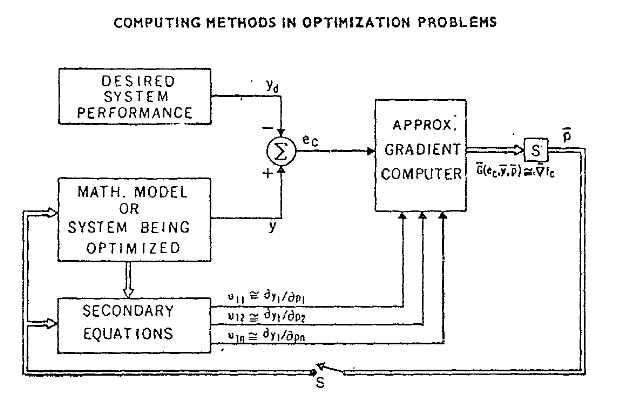
\includegraphics[height=0.3\textheight]{fig1.png}
    \caption{Schematic of Continuous Parameter Optimization Method}
    \label{fig:1}
\end{figure}

\begin{figure}
    \centering
    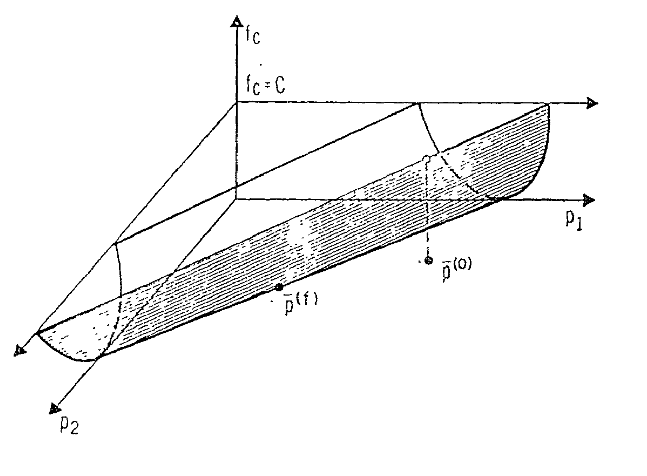
\includegraphics[height=0.3\textheight]{fig2.png}
    \caption{Instantaneous Criterion Surface}
    \label{fig:2}
\end{figure}


\subsection{The Gradient Vector}

\begin{equation}
    \nabla f_c = 2 {\left[ e_c u_{11}, \, e_c u_{12}, \, ... \, e_c u_{1m}\right]}'
\end{equation}

\begin{equation}
\begin{aligned}
     \vect{y}_d = A_d\vect{y}_d + B_d\vect{x} \hspace{1em} \vect{y}_d\left(0\right) = \vect{y}_{do} \\ \\
    A_d = 
{\begin{bmatrix}
    O & 1 \\
    -a_2 & -a_1
\end{bmatrix}},
B_d = {\begin{bmatrix}
    O & O \\
    a_3 & a_4
\end{bmatrix}},
\vect{x} = {\begin{bmatrix}
    x \\
    \vect{x}
\end{bmatrix}}
\end{aligned}
\end{equation}

\begin{equation}
    \vect{y} = A\vect{y} + Bx, \hspace{1em} \vect{y}\left(0\right) = \vect{y}_o
\end{equation}


% dummy page
\newpage
\thispagestyle{empty}
\centering
\topskip 0pt
\vspace*{\fill}
... skipped pages here ...
\vspace*{\fill}



% back to last page (labeled pg21)
\newpage % emulating the skipped pages, so pg 21 properly starts at top of page

% pages are skipped, need to reset the automatic numbering index for equations:
\setcounter{equation}{45} % set to the next eq # minus one (so the next is 46, as shown in the orig paper)
\setcounter{page}{21} % reset the page number because we skipped a range of pages

tr\begin{equation}
    \text{Placeholder 46}
\end{equation}

\begin{equation}
    \text{Placeholder 47}
\end{equation}

\begin{equation}
    \text{Placeholder 48}
\end{equation}

\begin{equation}
    \text{Placeholder 49}
\end{equation}

\begin{equation}
    \text{Placeholder 50}
\end{equation}

\begin{equation}
    \text{Placeholder 51}
\end{equation}

\begin{equation}
    \text{Placeholder 52}
\end{equation}






% Nothing in the References should be underlined. Can do!
\bibliographystyle{plain}
\bibliography{./bibliography.bib}



\end{document}
